\documentclass{article}

\usepackage{graphicx} % Required for inserting images
\usepackage{placeins}
\usepackage{amsfonts}
\usepackage{amsmath}
\usepackage{amsthm}
\usepackage{listings}
\usepackage{amssymb}
\usepackage[a4paper, left=1in, right=1in, top=1in, bottom=1in]{geometry}
\usepackage{xcolor}
\usepackage{tikz}
\usepackage{float}
\usepackage{caption}
\usepackage{booktabs}
\usetikzlibrary{automata, positioning, arrows.meta}

% Math Formatting
\renewcommand{\leq}{\leqslant}
\renewcommand{\geq}{\geqslant}
\renewcommand{\le}{\leqslant}
\renewcommand{\ge}{\geqslant}
\newcommand{\expect}{\mathbb{E}}
\newcommand{\prob}{\mathbf{P}}

% Custom Ruler
\newcommand{\ruler}{\bigskip\hrule\bigskip}
\newcommand{\bsq}{\hfill $\blacksquare$}

% Listings Configuration
\lstset{
    language=C++,          
    numbers=left,          
    numberstyle=\tiny\color{gray},  
    rulecolor=\color{black},         
    basicstyle=\ttfamily\footnotesize, 
    keywordstyle=\color{blue},   
    commentstyle=\color{green},  
    stringstyle=\color{red},   
    morekeywords={auto, register, inline}, 
}

\begin{document}

\subsection*{Problem 7: Skip Lists.} There are two subtasks here.

(a) Let's implement the skip list and compare it against any reputable built-in ordered map. Please design your own experiments. What are some questions you would like to know and how would you experimentally answer them?

\vspace{0.5em}
\hrule
\vspace{.5em}

\textbf{Answer to 7.a:}

\section{Introduction:}
This report examines the performance of a C++ skip list implementation through a series of experiments conducted on a MacOS system (Apple M3 chip). The experiments cover:
\begin{itemize}
    \item The comparison of two methods for simulating coin tosses (used in random level generation).
    \item An investigation into how varying the maximum height (or maximum level) affects the performance of skip lists.
    \item Performance benchmarks comparing skip list operations (insertion and search) with the standard C++ ordered set.
\end{itemize}
The following sections describe the experimental setup, present detailed results, and discuss the observed trends.

\section{Experimental Setup}
\textbf{System Configuration:}
\begin{itemize}
    \item \textbf{Processor:} Apple M3 (8-core: 4 performance cores up to 4.05\,GHz and 4 efficiency cores up to 2.75\,GHz).
    \item \textbf{Cache Hierarchy:}
    \begin{itemize}
        \item \textbf{L1 Cache:} Performance cores: 192\,KB (instruction) and 128\,KB (data); Efficiency cores: 128\,KB (instruction) and 64\,KB (data).
        \item \textbf{L2 Cache:} 16\,MiB (shared among performance cores for the M3/M3 Pro) and 32\,MiB for the M3 Max.
        \item \textbf{System Level Cache (SLC):} 8\,MiB integrated; extrapolated values for M3 Pro and M3 Max are approximately 12\,MiB and 48\,MiB, respectively.
    \end{itemize}
    \item \textbf{Memory:} LPDDR5-6400 with a bandwidth of 100\,GB/s.
\end{itemize}

\textbf{Compilation:} Benchmarks were compiled with \texttt{-O3} optimization using \textsf{clang 19.1.6}.

\section{Coin Toss Methods for Random Level Generation:}
The skip list requires random decisions (coin tosses) to determine the height of each node. Two methods were benchmarked:
\begin{enumerate}
    \item \textbf{Coin Flip For Real:} Simulates each coin toss individually.
    \item \textbf{Count Leading 0s:} Uses a fast bit-level method by counting the number of leading zeros in a random 32-bit integer.
\end{enumerate}

\subsection{Benchmark Results}
\begin{table}[H]
\centering
\small
\begin{tabular}{lrrr}
\hline
\textbf{Benchmark} & \textbf{Time (ns)}  & \textbf{Iterations} \\
\hline
Coin Flip For Real         & 25.7 & 26848418 \\
Coin Flip Count Leading 0s & 2.45 & 292785351 \\
\hline
\end{tabular}
\caption{The \textit{Count Leading 0s} method outperforms the standard coin-flip simulation by a large margin.}
\label{tab:coin_benchmarks}
\end{table}

\begin{figure}[H]
    \centering
    \begin{minipage}{0.32\textwidth}
        \centering
        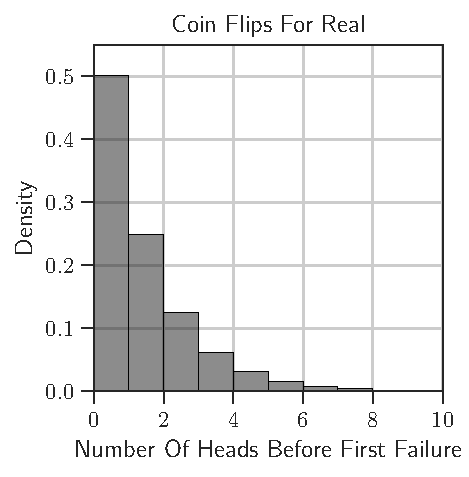
\includegraphics[width=\linewidth]{../notebook/plot/coin_flips_for_real.pdf}
        \caption*{Coin Flip For Real}
    \end{minipage}\hfill
    \begin{minipage}{0.32\textwidth}
        \centering
        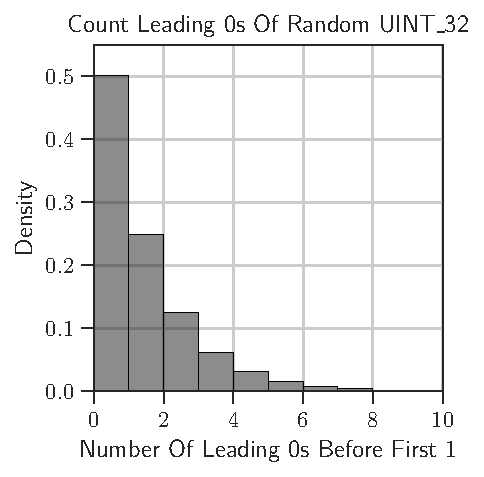
\includegraphics[width=\linewidth]{../notebook/plot/count_leading_0s_of_random_uint_32.pdf}
        \caption*{Count Leading 0s}
    \end{minipage}\hfill
    \begin{minipage}{0.32\textwidth}
        \centering
        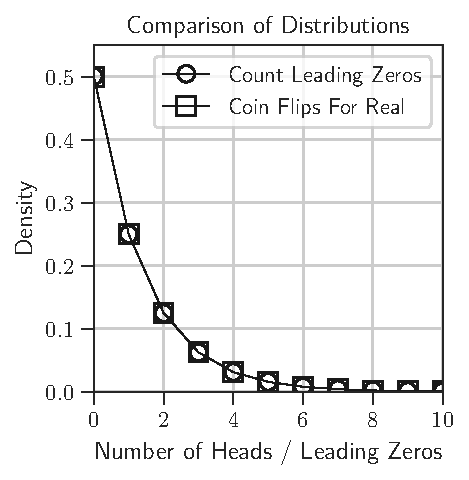
\includegraphics[width=\linewidth]{../notebook/plot/comparison_of_distributions.pdf}
        \caption*{Distribution Comparison}
    \end{minipage}
    \caption{Visual comparison of the two coin toss methodologies.}
    \label{fig:coin_toss_methods}
\end{figure}

From Figure 1 we can see that the simulation of coin flips by counting leading zeros is comparable to an actual coin flip simulation, but with significantly better performance.

\section{Impact of Varying Maximum Height}
The maximum level (height) of a skip list affects the balance between search speed and memory overhead. In the following experiments, the maximum level was varied while measuring CPU time and memory usage for both insertion and search operations.

\subsection{Experimental Data}
\begin{minipage}{0.5\textwidth}
    \centering
    \resizebox{1\textwidth}{!}{%
        \begin{tabular}{rrr}
        \hline
        \multicolumn{3}{c}{\textbf{Skip List Insertion}} \\ \hline
        Max Level & CPU Time (ms) & Memory Usage (KB) \\ \hline
        2  & 11000.61  & 4224 \\
        4  & 2363.20  & 688 \\
        6  & 676.20  & 2368 \\
        8  & 117.08  & 496 \\
        10 & 33.78  & 3040 \\
        12 & 25.01  & 2832 \\
        14 & 24.41  & 2832 \\
        16 & 22.37  & 2816 \\
        18 & 23.28  & 2032 \\
        20 & 23.87  & 3136 \\
        22 & 23.38  & 3424 \\
        24 & 23.86  & 2816 \\
        26 & 22.76  & 3056 \\
        28 & 24.80  & 2896 \\
        30 & 24.81  & 2816 \\
        32 & 25.10  & 3248 \\
        \hline
        \end{tabular}
    }
    \captionof{table}{Skip List Insertion Performance vs. \\Maximum Level}
    \label{tab:skiplist_maxlevel_insertion}
\end{minipage}\hfill
\begin{minipage}{0.5\textwidth}
    \centering
    \resizebox{1\textwidth}{!}{%
        \begin{tabular}{rrr}
        \hline
        \multicolumn{3}{c}{\textbf{Skip List Search}} \\ \hline
        Max Level & CPU Time (ms) & Memory Usage (KB) \\ \hline
        2  & 23331.85  & 448 \\
        4  & 5396.31  & 352 \\
        6  & 914.18  & 2592 \\
        8  & 109.63  & 2864 \\
        10 & 39.30  & 2800 \\
        12 & 26.00  & 2048 \\
        14 & 24.83  & 3056 \\
        16 & 23.67  & 3056 \\
        18 & 22.98  & 2032 \\
        20 & 22.92  & 3296 \\
        22 & 22.60  & 3056 \\
        24 & 25.35  & 3040 \\
        26 & 22.53  & 3056 \\
        28 & 24.45  & 3040 \\
        30 & 23.37  & 2816 \\
        32 & 23.22  & 2752 \\
        \hline
        \end{tabular}
    }
    \captionof{table}{Skip List Search Performance vs. \\Maximum Level}
    \label{tab:skiplist_maxlevel_search}
\end{minipage}


\subsection{Observations}
\begin{itemize}
    \item Lower maximum levels (e.g., 2 or 4) lead to significantly higher CPU times. 
    \item The memory usage seems to have outliers for insertion.
    \item Increasing the maximum level reduces CPU time until the benefit plateaus (diminishing returns).
    \item Both insertion and search operations follow similar trends with respect to the maximum level.
\end{itemize}
It is evident that the benefit in performance stops approximately around max level 12-14. Therefore for brevity, the next benchmarks all use a skip list of max level 20.

\begin{figure}[H]
    \centering
    \begin{minipage}{0.32\textwidth}
        \centering
        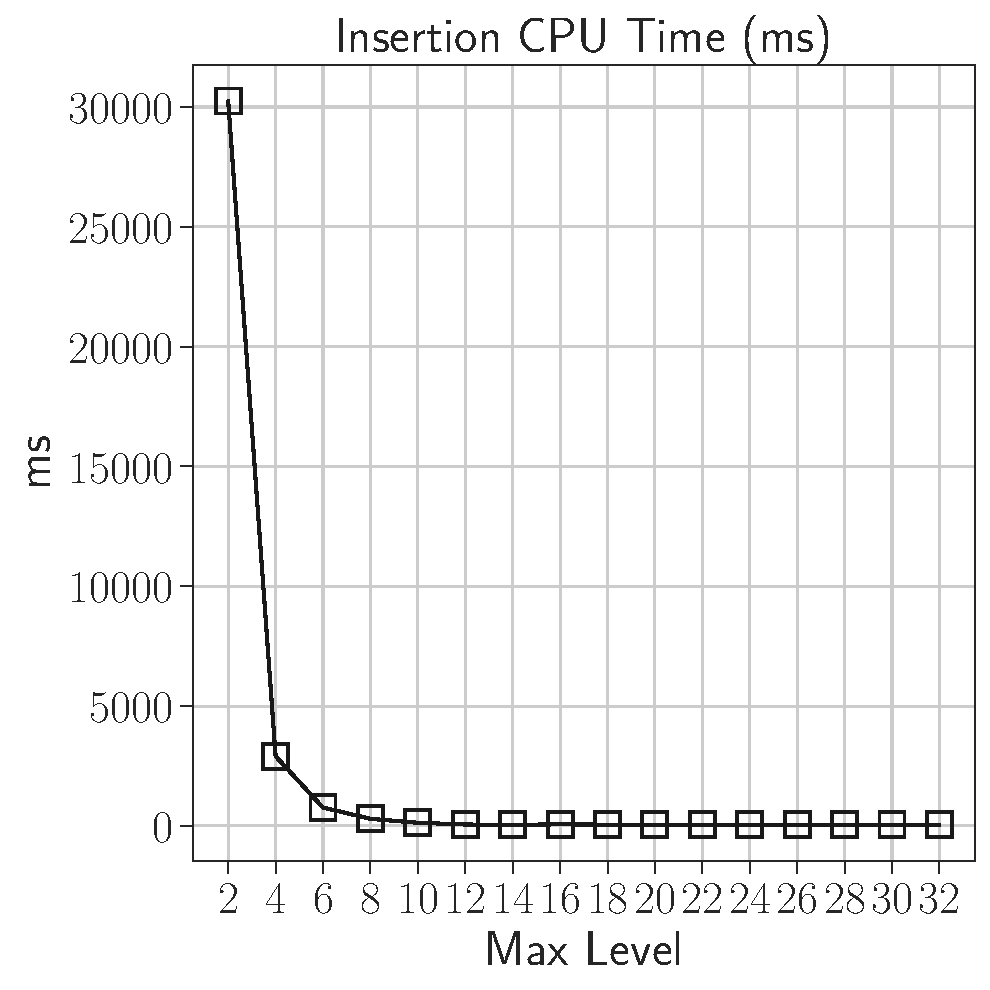
\includegraphics[width=\linewidth]{../notebook/plot/sl_maxlevel_insertion_cpu_time_(ms).pdf}
        \caption*{Insertion CPU Time}
    \end{minipage}\hfill
    \begin{minipage}{0.32\textwidth}
        \centering
        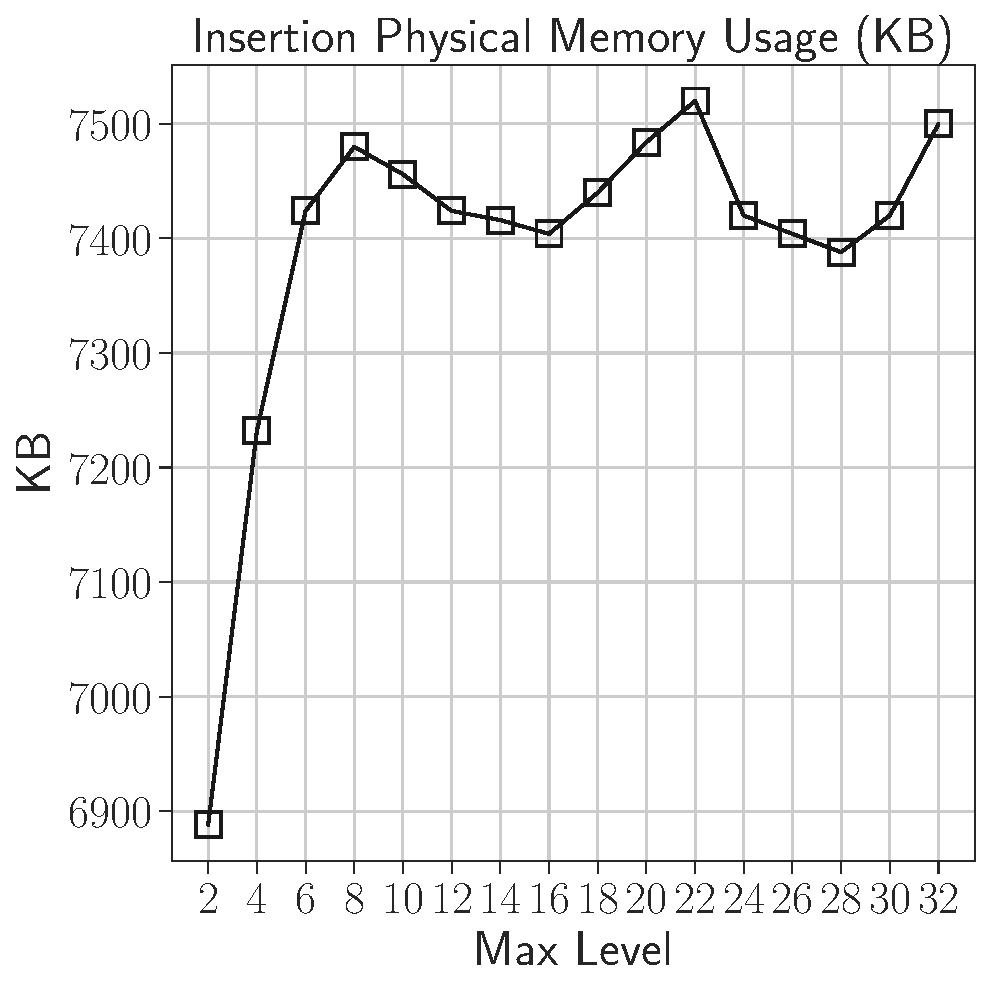
\includegraphics[width=\linewidth]{../notebook/plot/sl_maxlevel_insertion_physical_memory_usage_(kb).pdf}
        \caption*{Insertion Memory Usage}
    \end{minipage}\hfill
    \begin{minipage}{0.32\textwidth}
        \centering
        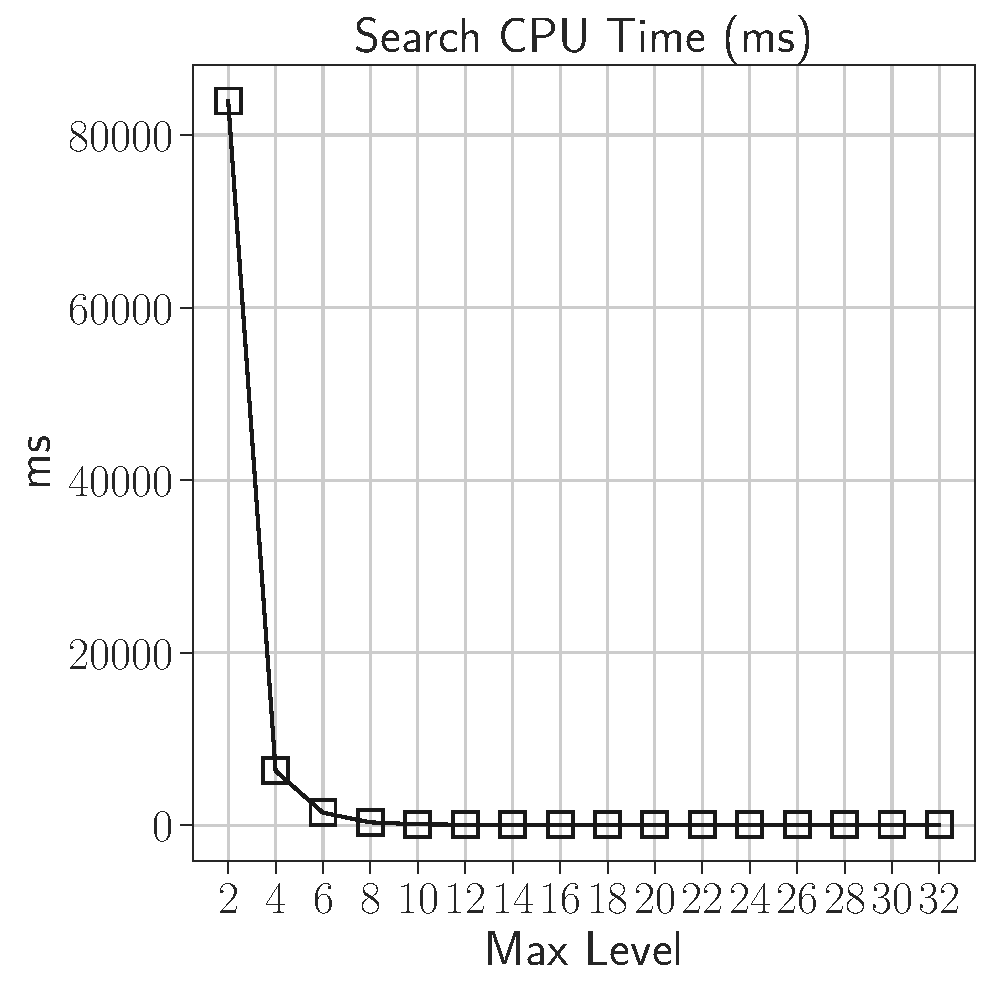
\includegraphics[width=\linewidth]{../notebook/plot/sl_maxlevel_search_cpu_time_(ms).pdf}
        \caption*{Search CPU Time}
    \end{minipage}
    \caption{Performance of skip list operations as the maximum level varies.}
    \label{fig:skiplist_maxlevel}
\end{figure}

\section{Skip List vs. Ordered Map Performance}

This section presents the performance comparison between Skip List (Max Level 20) and Ordered Map in terms of insertion and search operations.

\FloatBarrier
\begin{table}[h]
    \centering
    \begin{minipage}{0.48\textwidth}
        \centering
        \caption{Skip List Insertion Performance}
        \begin{tabular}{rr}
            \toprule
            \textbf{n} & \textbf{CPU Time (ms)} \\
            \midrule
            8       & 1.14E-04  \\
            16      & 1.76E-04  \\
            32      & 5.78E-04  \\
            64      & 1.20E-03  \\
            128     & 3.25E-03  \\
            256     & 6.63E-03  \\
            512     & 1.60E-02  \\
            1024    & 6.98E-02  \\
            2048    & 2.00E-01  \\
            4096    & 4.39E-01  \\
            \bottomrule
        \end{tabular}
        \label{tab:sl_insertion}
    \end{minipage}%
    \hfill
    \begin{minipage}{0.48\textwidth}
        \centering
        \caption{Ordered Map Insertion Performance}
        \begin{tabular}{rr}
            \toprule
            \textbf{n} & \textbf{CPU Time (ms)} \\
            \midrule
            8       & 0.00E+00  \\
            16      & 0.00E+00  \\
            32      & 0.00E+00  \\
            64      & 1.32E+01  \\
            128     & 4.73E+00  \\
            256     & 1.25E+01  \\
            512     & 0.00E+00  \\
            1024    & 5.78E+00  \\
            2048    & 8.72E+00  \\
            4096    & 1.45E+01  \\
            \bottomrule
        \end{tabular}
        \label{tab:om_insertion}
    \end{minipage}
\end{table}

\begin{table}[h]
    \centering
    \begin{minipage}{0.48\textwidth}
        \centering
        \caption{Skip List Search Performance}
        \begin{tabular}{rr}
            \toprule
            \textbf{n} & \textbf{CPU Time (ms)} \\
            \midrule
            8       & 2.90E-05  \\
            16      & 8.50E-05  \\
            32      & 3.49E-04  \\
            64      & 6.10E-04  \\
            128     & 1.22E-03  \\
            256     & 2.70E-03  \\
            512     & 7.12E-03  \\
            1024    & 6.00E-02  \\
            2048    & 1.57E-01  \\
            4096    & 3.99E-01  \\
            \bottomrule
        \end{tabular}
        \label{tab:sl_search}
    \end{minipage}%
    \hfill
    \begin{minipage}{0.48\textwidth}
        \centering
        \caption{Ordered Map Search Performance}
        \begin{tabular}{rr}
            \toprule
            \textbf{n} & \textbf{CPU Time (ms)} \\
            \midrule
            8       & 3.20E-05  \\
            16      & 9.40E-05  \\
            32      & 2.00E-04  \\
            64      & 4.30E-04  \\
            128     & 9.84E-04  \\
            256     & 2.25E-03  \\
            512     & 6.70E-03  \\
            1024    & 3.84E-02  \\
            2048    & 1.09E-01  \\
            4096    & 2.51E-01  \\
            \bottomrule
        \end{tabular}
        \label{tab:om_search}
    \end{minipage}
\end{table}
\FloatBarrier



\section{Conclusion}
The experiments demonstrate that:
\begin{itemize}
    \item The \textbf{Count Leading 0s} method greatly improves the performance of random level generation compared to simulating individual coin flips.
    \item Skip lists exhibit competitive performance in both insertion and search operations when compared to an ordered map, although the performance trade-offs differ by operation.
    \item Adjusting the maximum level of the skip list can optimize performance—lower levels incur higher costs, while higher levels improve speed up to a point.
\end{itemize}


$\hfill$ \(\blacksquare\)

\vspace{0.5em}
\hrule
\vspace{1em}

(b) Searching in a skip list typically starts from the top-left corner. In this way, a search takes $O(\log n)$ whp., where $n$ is the number of keys stored in the skip list. If we keep bi-directional pointers for each vertical column, we will be able to go up and down any column freely. This allows us to start from the smallest key and work our way to the desired key.

You'll extend the skip list in the following way. Maintain a "pointer" to the smallest key. Make up/down pointers bi-directional. Design and implement a search algorithm that runs in $O(\log d)$ time, where $d$ is the number of elements smaller than the key you're searching for.

\vspace{0.5em}
\hrule
\vspace{.5em}

\textbf{Answer to 7.b:}

$\hfill$ \(\blacksquare\)

\vspace{0.5em}
\hrule
\vspace{1em}

\bsq

\end{document}
